\chapter{Marco teórico}
\label{ch:marco}


\section{Péndulo amortiguado a hélice PAMH}

El péndulo amortiguado a hélice corresponde a una planta de laboratorio compuesta de un motor con hélice controlado por torque, una masa pequeña, péndulo y soportes de aluminio de baja fricción. Un modelo simplificado del sistema se muestra en la Figura \ref{fig:modpen} \textcolor{SkyBlue}{PAMH1}.

\begin{figure}[h]
	\centering
	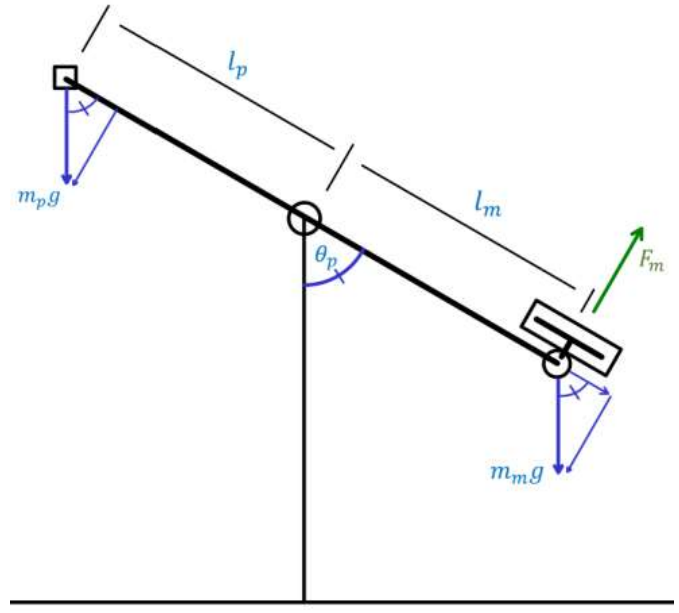
\includegraphics[scale=0.3]{fig/new/ModeloPendulo.png}
	\caption{Modelo simplificado del PAMH.}
	\label{fig:modpen}
\end{figure}

El objetivo de dicho sistema es controlar la magnitud del ángulo $\theta_p$, únicamente ejerciendo torque al accionar a una distancia $l_m$ el motor con una fuerza $F_m$ y movimiento de su masa $m_m$, mientras a una distancia de $l_p$ del centro se encuentra una masa $m_p$ que contrarresta el movimiento.

De manera que al analizar el sistema con sumatoria de torques se obtiene la constante de rosamiento central $B$ (en caso de existir) junto con la inercia ejercida $J_p$. Por lo tanto, se definen las variables de estado siguientes y sus ecuaciones de estado mostradas en \ref{ecu:ecuestados} \textcolor{SkyBlue}{ControlModerno}.

\[x_1 = \theta_p \qquad x_2 = \dot{\theta}_p \qquad y = x_1 = \theta_p\]
\begin{equation}
	\left \{ \begin{array}{lcc} \dot{x}_1 = x_2 \\ \\ \dot{x}_2 = -\dfrac{B}{J_p} x_2 + (m_p l_p -m_m l_m)\dfrac{g}{J_p}sen(x_1) +\dfrac{l_m}{J_p}F_m \end{array} \right.
	\label{ecu:ecuestados}
\end{equation}




\section{Aprendizaje reforzado RL}


Al estudiar el concepto de aprendizaje reforzado y los diferentes métodos y algoritmos que corresponden a este tipo de aprendizaje automático, se obtiene el resumen de la Figura \ref{fig:teoriaRL}, en donde se muestra que las principales secciones son el RL basado en modelo y el libre de modelo. De igual forma se cuenta con el aprendizaje reforzado profundo (DRL), una combinación y reestructuración de métodos de cada subdivisión \textcolor{SkyBlue}{DataScience}.

\begin{figure}[hh]
	\centering
	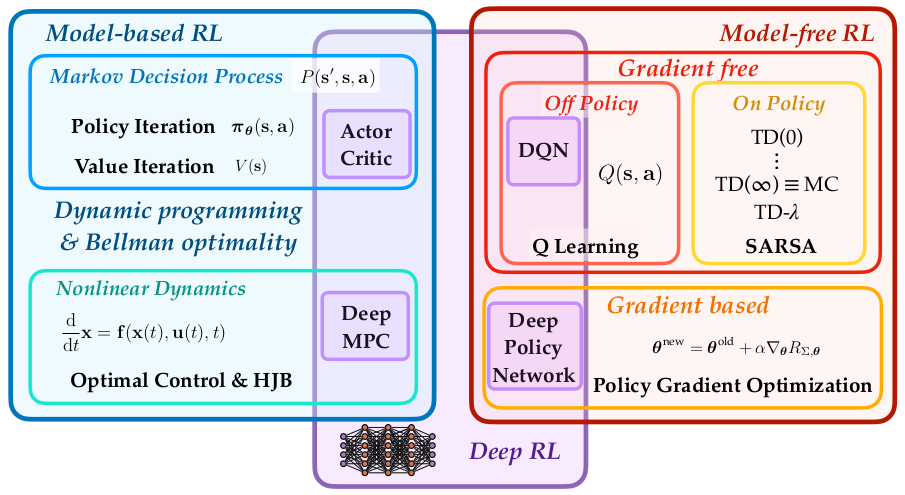
\includegraphics[scale=0.35]{fig/new/CatRL.png}
	\caption{Resumen de categorización del RL \textcolor{SkyBlue}{DataScience}.}
	\label{fig:teoriaRL}
\end{figure}


De igual manera, los avances en la investigación de diferentes métodos como las redes neuronales recurrentes (RNN), ejemplificado por Mamba \textcolor{SkyBlue}{Mamba}, ha mostrado la capacidad de optimización del desempeño de estas para llegar a competir con los modelos basados en \textit{Transformer}.


\subsection*{Control predictivo del modelo (MPC)}

La estructura de comunicación entre el sistema y el modelo de control mediante maching learning se efectua con base en funciones de optimización, donde se generan acciones controladas en cada paso para controlar alguna característica ($\mathbf{\hat{F}}$) y se toma la primera muestra de dicha acción ($\hat{x}_{k+1}$) para variar la respuesta del controlador enviada al sistema ($\mathbf{u}_j$), esto independiente y apllicable a sistemas lineales o no lineales. El proceso se simplifica en la Fig. \ref{fig:mpc}.


\begin{figure}[h]
	\centering
	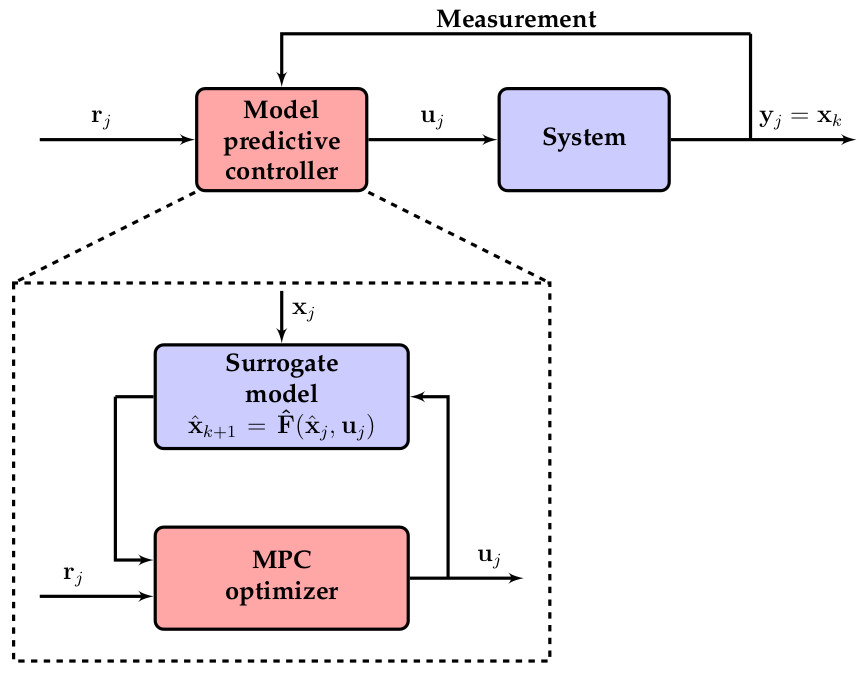
\includegraphics[scale=0.35]{fig/MPC.png}
	\caption{Esquemático del control predictivo del modelo (MPC) \textcolor{SkyBlue}{DataScience}.}
	\label{fig:mpc}
\end{figure}








\begin{comment}

%References

@article{PAMH1,
author = {Castaño Hernández, A. and Moreno Beltrán, J. P. and Hernández Pérez, J. F. and Villafuerte Segura, R.},
year = {2018},
title = {Diseño y control de un sistema balancín con motor y hélice de bajo costo},
journal = {ICBI},
volume = {5},
numbre = {10},
doi = {https://doi.org/10.29057/icbi.v5i10.2937}
}

@article{Mamba,
author = {Gu, Albert and Dao, Tri},
year = {2023},
title = {Mamba: Linear-Time Sequence Modeling with Selective State Spaces},
journal = {Cornell University, Arxiv},
doi = {https://doi.org/10.48550/arXiv.2312.00752}
}

\end{comment}



\section{*************************************************}







